% !TeX root = ../Skript_DB.tex
\cohead{\Large\textbf{Anlegen einer DB}}
\cohead{\Large\textbf{Anlegen/Befüllen einer DB}}
\subsection[Anlegen/Befüllen einer DB]{SQL - Anlegen und Befüllen einer Datenbank}
Erinnerung: Wir werden das Programm SQLite als Datenbankmanagementsystem (DBMS) verwenden. Nach dem Starten von SQLite sind nur noch SQLite-spezifische Befehle, die immer mit einem Punkt beginnen oder SQL-Anweisungen erlaubt.

\subsection{Erstellen bzw. Öffnen einer Datenbank}
\begin{wrapfigure}{r}{6.91cm}
	\centering
	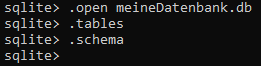
\includegraphics[]{\pics/createDB.png}
	\caption*{Da noch keine Tabellen angelegt sind, geben die Befehle \lstinline!.tables! und \lstinline!.schema! keine Ausgabe zurück.}
\end{wrapfigure}
Starte die \texttt{sqlite3.exe}. Mit dem Befehl \lstinline!.open #Name#.db! (z.B. \lstinline!.open meineDatenbank.db!) lässt sich eine bestehende DB öffnen bzw. neu erstellen. Im Verzeichnis, in dem auch \texttt{sqlite3.exe} liegt, sollte nun (falls zuvor noch nicht vorhanden) eine neue Datei \texttt{\#Name\#.db} erstellt worden sein.

Mit dem Befehl \lstinline!.tables! kann man sich alle in der DB vorhandenen Tabellen/Entitätstypen anzeigen lassen.

Mit dem Befehl \lstinline!.schema! kann man sich die Tabellen mit einer Liste der Attribute anzeigen lassen.
\begin{tcolorbox}[title=Datenbank öffnen]
	Starte \texttt{sqlite3.exe} und gib dann \lstinline!.open datenbankname.db! ein.
\end{tcolorbox}

\subsection{Erstellen bzw. löschen von Tabellen/Entitätstypen}
Neue Tabellen/Entitätstypen lassen sich mit dem SQL-Befehl \lstinline!CREATE TABLE! erzeugen:

\begin{tcolorbox}[title=Tabellen erstellen]
	\lstinline[breaklines=true]!CREATE TABLE name_tabelle (name_attribut1 datentyp1 einschränkung1, name_attribut2 datentyp2 einschränkung2, ...);!
\end{tcolorbox}
\textcolor{red}{ACHTUNG: Bei SQL-Befehlen den Strichpunkt am Ende der Zeile nicht vergessen!} Man kann SQL-Befehle auch auf mehrere Zeilen aufteilen.

Als Datentypen werden wir \lstinline!INT! für ganze Zahlen und \lstinline!TEXT! für Texte oder Geburtsdaten verwenden. Dem interessierten Leser seien die restlichen Datentypen zum Selbststudium ans Herz gelegt.

Als Einschränkungen werden wir uns auf \lstinline!PRIMARY KEY! und \lstinline!NOT NULL! beschränken. \lstinline!PRIMARY KEY! markiert das Attribut als Primärschlüssel und sollte als erstes Attribut angelegt werden. \lstinline!NOT NULL! zeigt an, dass dieses Attribut beim Füllen der Tabelle mit Daten nicht leer bleiben darf. Die Angabe von Einschränkungen ist optional.

Bestehende Tabellen lassen sich mit dem Befehl \lstinline!DROP TABLE name_tabelle! wieder löschen:
\begin{tcolorbox}[title=Tabellen löschen]
	\lstinline[breaklines=true]!DROP TABLE name_tabelle !
\end{tcolorbox}
\begin{figure}[h]
	\centering
	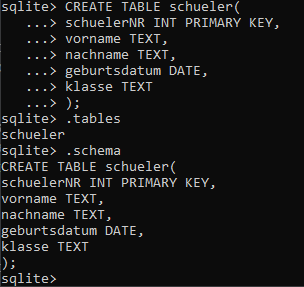
\includegraphics[]{\pics/createTable_schueler.png}
	\caption*{Die Tabelle \lstinline!schueler! wurde angelegt. Die Befehle \lstinline!.tables! und \lstinline!.schema! haben nun einen Rückgabewert.}
\end{figure}
\begin{figure}[h]
	\centering
	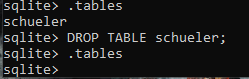
\includegraphics[]{\pics/dropTabel_schueler.png}
	\caption*{Die Tabelle \lstinline!schueler! wurde gelöscht.}
\end{figure}

\subsection{Befüllen einer Tabelle mit Daten}
Um einer Tabelle eine neue Entität/Zeile hinzuzufügen, verwendet man den \lstinline!INSERT INTO! Befehl:

\begin{tcolorbox}[title=Befüllen einer Tabelle]
	\lstinline!INSERT INTO name_tabelle VALUES(wert1, wert2, wert3, ...);!
\end{tcolorbox}
\begin{itemize}
	\item Alle Attribute angegeben: Sollen für alle Attribute Werte angegeben werden, so kann man einfach die Werte als kommaseparierte Liste angeben:\\
	\lstinline!INSERT INTO schueler VALUES(1,'Heinz','Huber','01.01.2000','BKFH');!

	Beachte, dass Texte mit Anführungszeichen (neben dem \#-Zeichen) angegeben werden müssen.
	\item Manche Attribute ohne Wert: Hat man für manche Attribute keinen Wert zur Hand, so kann man die Entität trotzdem anlegen, indem man hinter den Namen der Entität die Liste der Attribute angibt, für die man Werte zur Hand hat:

	\lstinline!INSERT INTO schueler(schuelerNR, vorname, nachname, klasse) VALUES (20,!

	\lstinline!'Anton', 'Atonovich', 'BK11');!
\end{itemize}

\begin{Exercise}[title={Beantworte folgende Fragen mit Hilfe deiner Datenbank.}, label=Befuellen]
	\begin{enumerate}
		\item Erzeuge eine Tabelle \lstinline!schueler! mit den Attributen \lstinline!schuelerNR! als Primärschlüssel, der nicht NULL sein darf, \lstinline!name!, \lstinline!plz! und \lstinline!klasse!.
		\item Füge 2 verschiedene Schüler hinzu, die aus den Klassen BK13 und BK21 stammen.
		\item Was passiert, wenn man einen weiteren Schüler mit einer bereits vergebenen \lstinline!schuelerNR! hinzufügen will?
		\item Was passiert, wenn man einen weiteren Schüler einfügen will ohne eine \lstinline!schuelerNR! anzugeben?
		\item Wie sehen die Ausgaben von \lstinline!.tables! und \lstinline!.schema! aus?
	\end{enumerate}
\end{Exercise}
%%%%%%%%%%%%%%%%%%%%%%%%%%%%%%%%%%%%%%%%%
\begin{Answer}[ref=Befuellen]
	\begin{enumerate}
		\item Erzeuge eine Tabelle \lstinline!schueler! mit den Attributen \lstinline!schuelerNR! als Primärschlüssel, der nicht NULL sein darf, \lstinline!name!, \lstinline!plz! und \lstinline!klasse!.

		\lstinline[breaklines=true]!CREATE TABLE schueler(schuelerNR INT PRIMARY KEY NOT NULL, name TEXT, plz INT, klasse TEXT);!
		\item Füge 2 verschiedene Schüler hinzu, die aus den Klassen BK13 und BK21 stammen., z.B.:

		\lstinline!INSERT INTO schueler VALUES (1, 'Heinz Huber', 70180, 'BK13');!

		\lstinline!INSERT INTO schueler VALUES (2, 'Dasan Ilhan', 70567, 'BK21');!

		\item Was passiert, wenn man einen weiteren Schüler mit einer bereits vergebenen schuelerNR hinzufügen will?

		Z.B. folgender Befehl: \lstinline!INSERT INTO schueler VALUES (1, 'Alina Lutz', 70874, 'BK21');!
		Es wird ein Fehler ausgegeben: \lstinline!Runtime error: UNIQUE constraint failed: schueler.schuelerNR!

		Unique bedeutet einzigartig und constraint steht für Einschränkung. Der Fehler besagt also, dass beim Hinzufügen eines Schülers in der Tabelle \lstinline!schueler! der Wert des Attributs \lstinline!schuelerNR! nicht einzigartig war.
		\item Was passiert, wenn man einen weiteren Schüler mit der schuelerNR NULL einfügen will?

		Z.B. folgender Befehl: \lstinline!INSERT INTO schueler(name) VALUES ('Vanessa Oranbay');!. Dieser Befehl würde gerne eine Zeile in der Tabelle \lstinline!schueler! anlegen, bei der alle Einträge bis auf den \lstinline!name! den Wert NULL haben.
		Es wird ein Fehler ausgegeben: \lstinline!Runtime error: NOT NULL constraint failed: schueler.schuelerNR!

		Der Fehler besagt also, dass beim Hinzufügen eines Schülers in der Tabelle \lstinline!schueler! der Wert des Attributs \lstinline!schuelerNR! NULL war, was nicht erlaubt ist.
		\item Wie sehen die Ausgaben von .tables und .schema aus?

		\lstinline!sqlite> .table!

		\lstinline!schueler!

		\lstinline!sqlite> .schema!

		\lstinline!CREATE TABLE schueler(schuelerNR INT PRIMARY KEY NOT NULL,!

		\lstinline!name TEXT, plz INT, klasse TEXT);!
	\end{enumerate}
\end{Answer}